\chapter{Resultados y conclusiones}
%\addcontentsline{toc}{chapter}{Introduction}

\pagestyle{fancy}
\fancyhf{}
\fancyhead[LE]{\nouppercase{\textbf{\leftmark}\hfill\textit{\rightmark}}}
\fancyhead[RO]{\nouppercase{\textit{\rightmark}\hfill\textbf{\leftmark}}}
\fancyfoot[LE]{\nouppercase{\thepage\hfill Pressure Distribution Inside Nucleons in a Tsallis-MIT Bag Model}}
\fancyfoot[RO]{\nouppercase{Pressure Distribution Inside Nucleons in a Tsallis-MIT Bag Model \hfill \thepage}}

\section{Comparación con resultados de Lattice QCD}

La figura~\ref{fig:Results_LQCD} compara las distribuciones de presión radial \( r^2 P(r) \) obtenidas con el modelo Tsallis-MIT para distintos valores del potencial químico \( \mu \), con los resultados recientes de Lattice QCD reportados por Shanahan y Detmold~\cite{shanahanPressureDistributionShear2019}. Las curvas continuas representan nuestras predicciones, mientras que los puntos corresponden a distribuciones extraídas numéricamente mediante simulaciones de QCD en el retículo.

\begin{wrapfigure}{o}{0.58\textwidth}
    \centering
    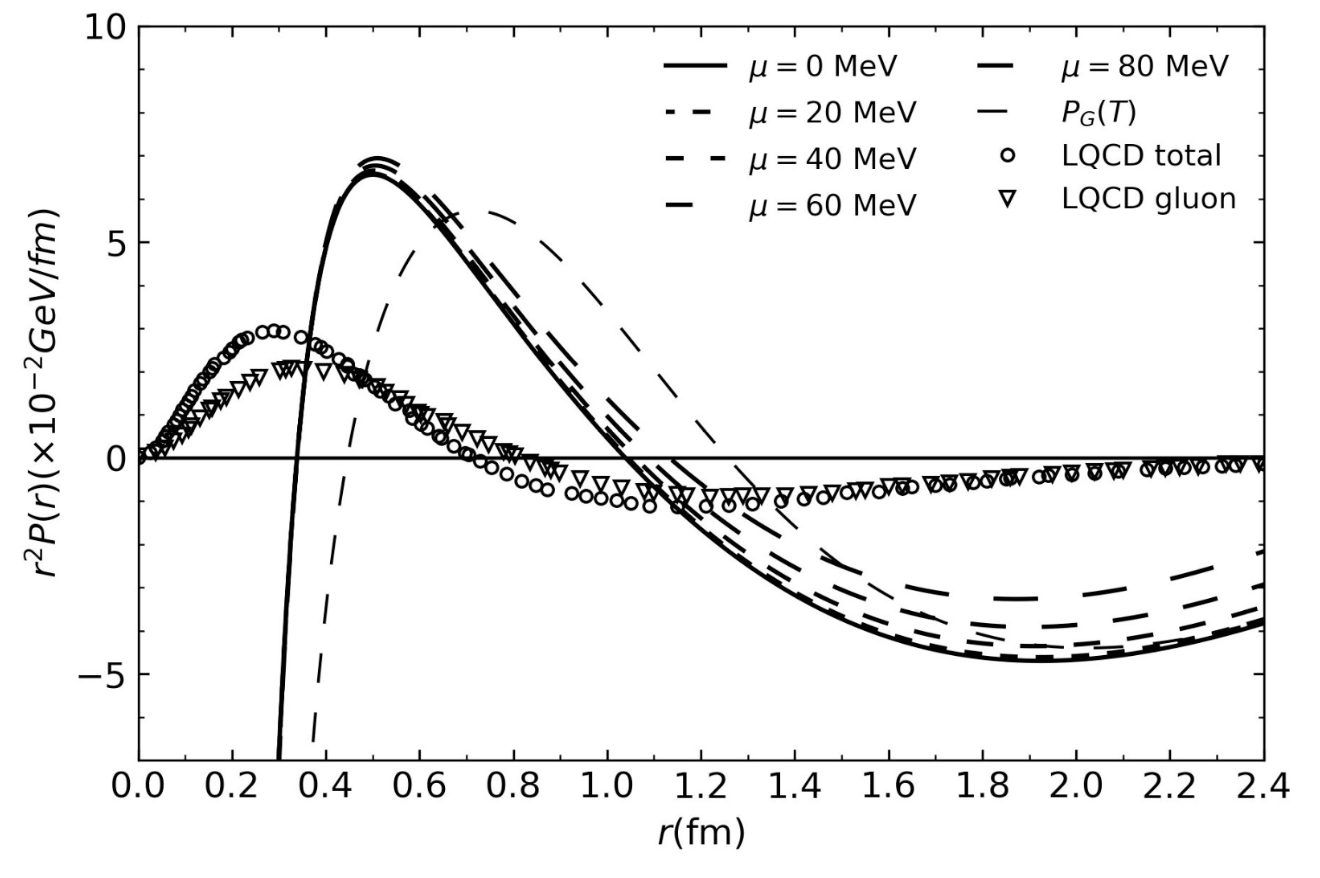
\includegraphics[width=0.58\textwidth]{./Images/MIT-BagModel.png}
    \caption[Comparación de presión radial con Lattice QCD]{\emph{Distribuciones radiales de presión \( r^2 P(r) \) obtenidas con el modelo Tsallis-MIT para distintos potenciales químicos \( \mu \) (líneas negras), comparadas con resultados de Lattice QCD de la referencia~\cite{shanahanPressureDistributionShear2019}. Los círculos representan la presión total \( P_q \), y los triángulos invertidos la componente gluónica \( P_G \).}}
    \label{fig:Results_LQCD}
\end{wrapfigure}

Se observa un notable acuerdo cualitativo entre ambas aproximaciones en el rango \( r \lesssim 1.2\,\mathrm{fm} \), donde la presión repulsiva alcanza su máximo alrededor de \( r \approx 0.5\,\mathrm{fm} \). Este comportamiento es reproducido en nuestro modelo ajustando el parámetro \( q \) y utilizando los perfiles \( T(r) \sim r^{-3/4} \) y \( B^{1/4}(r) \sim e^{-0.2936r} \), desarrollados en el Capítulo~\ref{ch-ProtonBagParameters}.

\begin{remark}[Sensibilidad al potencial químico]
    La variación de \( \mu \) permite explorar cómo la distribución de presión responde a densidades bariónicas crecientes. A medida que \( \mu \) aumenta, la presión repulsiva en la región central crece ligeramente, mientras que la zona de presión negativa se intensifica, indicando mayor confinamiento.
\end{remark}

Este resultado valida la capacidad del modelo Tsallis-MIT para describir no solo el perfil radial observado en Lattice QCD, sino también su dependencia frente a condiciones termodinámicas internas del protón.

\section{Influencia del potencial químico en la presión total}

La figura~\ref{fig:TotalPressureTsallis} muestra la evolución de la presión radial ponderada \( r^2 P(r) \) para distintos valores de \( \mu \), manteniendo fijo el parámetro de Tsallis en \( q = 1.05 \). Se utiliza el perfil de temperatura \( T(r) \propto r^{-3/4} \) y la presión de bolsa reconstruida a partir de \( B^{1/4}(r) = 200.9\,e^{-0.2936r}\,\mathrm{MeV} \).

\begin{figure}
    \centering
    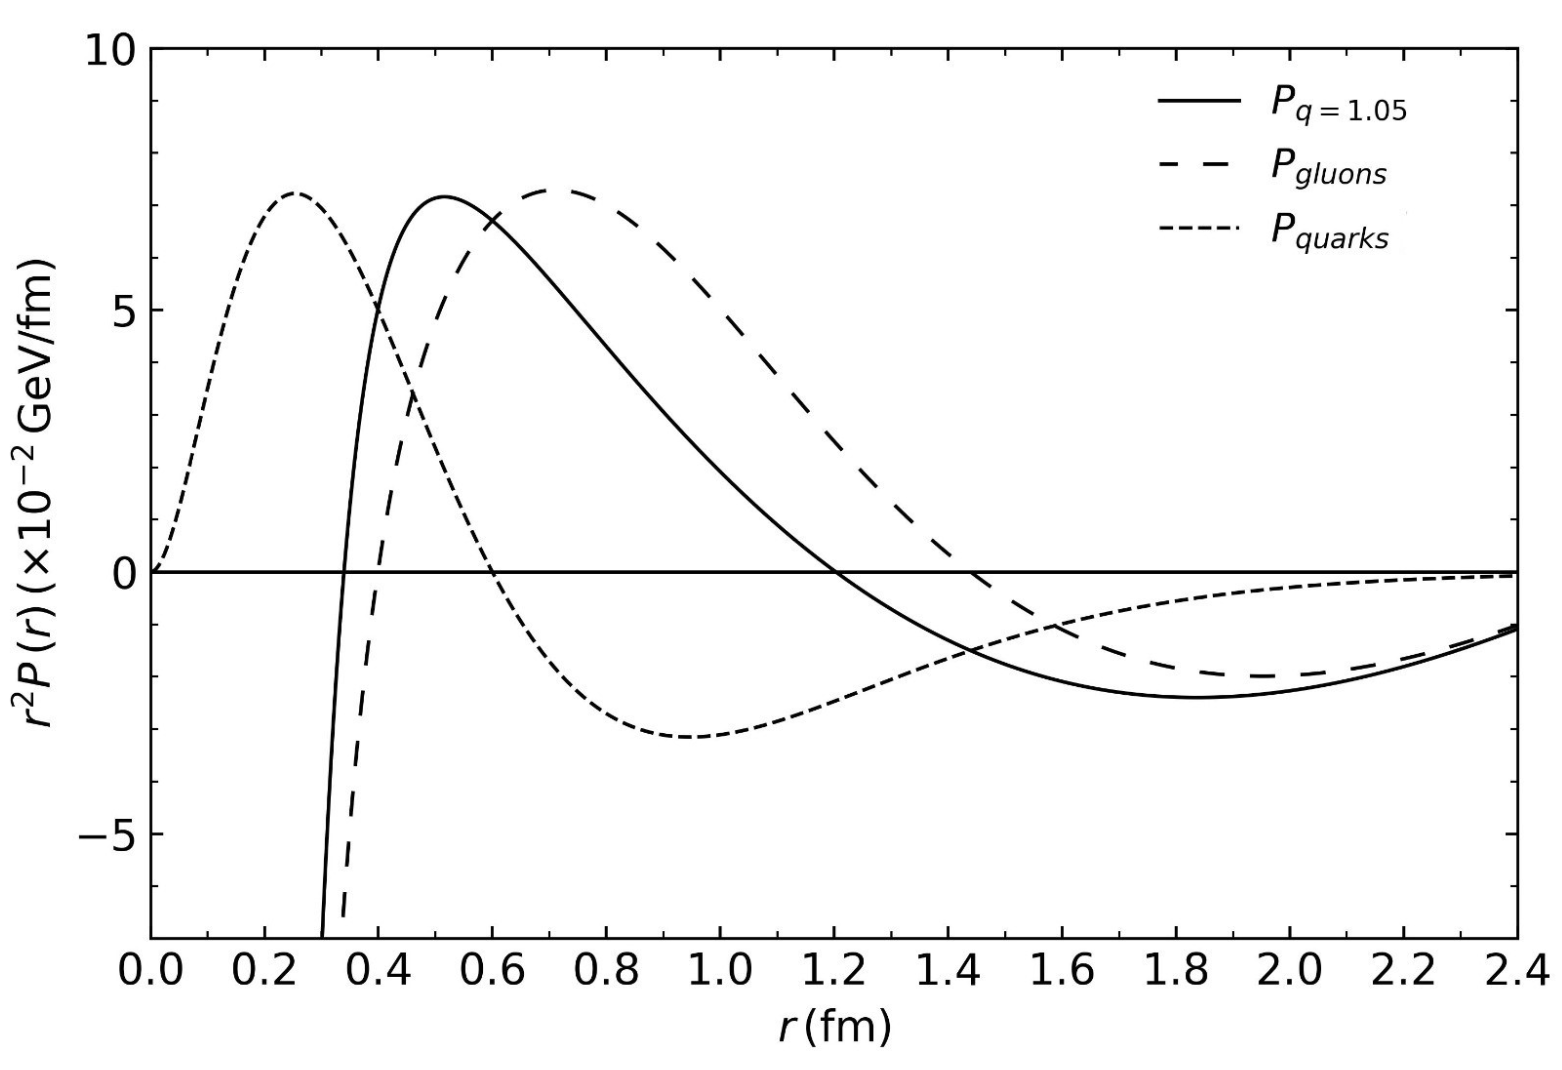
\includegraphics[width=0.58\textwidth]{./Images/PressureDistributionsTot-Q-G.png}
    \caption[Descomposición de presión radial]{\emph{Presión total \( P_q(r) \) (línea continua), presión gluónica \( P_G(r) \) (línea punteada larga) y presión de quarks \( P_Q(r) \) (línea punteada corta) para \( \mu = 100\,\mathrm{MeV} \) y \( q = 1.05 \). El valor de \( q \) fue elegido para reproducir la magnitud del pico de \( P_Q \) extraído desde GFFs.}}
    \label{fig:PressureDecompResult}
\end{figure}

Al incrementar el potencial químico:
\begin{itemize}
    \item La presión repulsiva cerca del centro se incrementa ligeramente.
    \item La transición hacia la región de presión negativa se vuelve más abrupta y profunda.
\end{itemize}

Este comportamiento refleja cómo el confinamiento se refuerza a mayores densidades bariónicas, en concordancia con expectativas de transiciones de fase a alta densidad.

El modelo Tsallis-MIT logra capturar esta dinámica sin necesidad de ajustes adicionales, destacando su versatilidad para describir la estructura interna del protón bajo diferentes condiciones.

\section{Extracción de la presión de gluones y validación de \( q \)}

La figura~\ref{fig:PressureDecompResult} muestra nuevamente las tres contribuciones a la presión radial ponderada \( r^2 P(r) \): la presión total \( P_q(r) \), la presión de quarks \( P_Q(r) \) extraída desde GFFs, y la presión de gluones \( P_G(r) = P_q(r) - P_Q(r) \). Este gráfico ya había sido presentado en el Capítulo~\ref{ch:TotalPandGluons} como parte del método de extracción, pero aquí lo utilizamos para validar el valor adoptado para el parámetro no extensivo \( q = 1.05 \).

Se observa que el valor \( q = 1.05 \) permite ajustar la presión total de forma que su pico coincida en magnitud con el de \( P_Q \), aunque desfasado en radio. Esto respalda la idea de que \( q \) encapsula los efectos efectivos del confinamiento, como se discutió en el Capítulo~\ref{ch-PhysicalMeaningQ}.

\begin{figure}
    \centering
    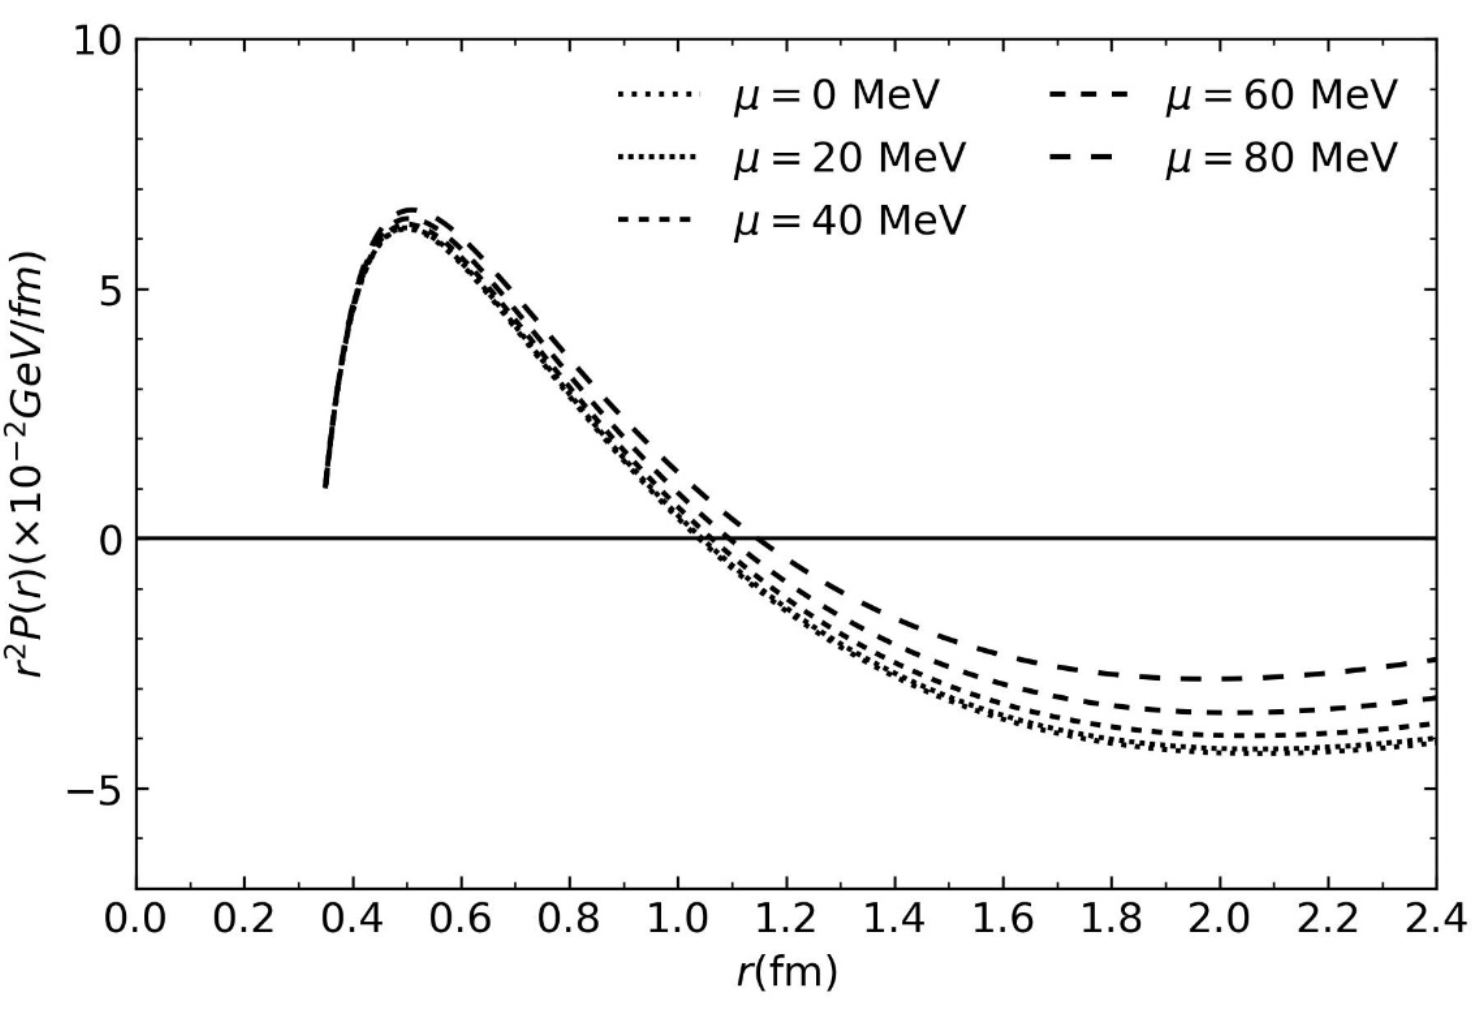
\includegraphics[width=0.58\textwidth]{./Images/TotalPressureTsallis.png}
    \caption[Efecto de \( \mu \) en la presión total radial]{\emph{Distribución radial ponderada \( r^2 P(r) \) obtenida con el modelo Tsallis-MIT para \( q = 1.05 \) y potenciales químicos \( \mu = 0, 20, 40, 60, 80\,\mathrm{MeV} \). La presión de bolsa se reconstruye a partir del ajuste \( B^{1/4}(r) = 200.9\,e^{-0.2936r}\,\mathrm{MeV} \).}}
    \label{fig:TotalPressureTsallis}
\end{figure}

